
%(BEGIN_QUESTION)
% Copyright 2010, Tony R. Kuphaldt, released under the Creative Commons Attribution License (v 1.0)
% This means you may do almost anything with this work of mine, so long as you give me proper credit

This newly-installed FOUNDATION Fieldbus H1 segment has a problem.  Flow transmitter FT-31 does not communicate with the host (DCS), while all other other field instruments on this segment do.  None of the transmitters have been connected to their respective processes yet -- just their spur cables to the network segment to check for communication:

$$\includegraphics[width=15.5cm]{i04729x01.eps}$$

You are asked to diagnose the problem as best you can.  Unfortunately, you have absolutely no test equipment with you at the time: only some basic hand tools (wrenches, screwdrivers, etc.).  Neither do you have access to the host system (a Honeywell Experion DCS) to check network diagnostic statistics.  All you have is the operator's observation (over radio) back at the control room, telling you whether or not FT-31 is ``on line'' and communicating.

Devise a useful diagnostic test you could perform on this new system to at least identify {\it where} the problem is located that is causing FT-31 to not communicate.  In order to receive full credit, your proposed test must positively identify the general location of the fault regardless of its outcome.  An example of a poor test would be something like ``check for loose wire connections at the transmitter'' because if that test revealed tight wire connections, you would still have no idea where the problem was located.

\vskip 50pt

\underbar{file i04729}
%(END_QUESTION)





%(BEGIN_ANSWER)

Full credit for a test where any outcome is positively informative.  If the proposed test merely checks for one possible fault (e.g. the loose wire connections), award only 2 points.

\vskip 10pt

The simplest way to test this system is to move FT-31 to another physical location on the segment.  If the problem moves with FT-31 (to the new location), then the problem has to do with FT-31 specifically (e.g. bad transmitter, address being skipped by host FUN/NUN, etc.).  If the problem remains at FT-31's old location, the problem has to do with that location (e.g. bad spur cable, coupling device port, etc.).

%(END_ANSWER)





%(BEGIN_NOTES)

{\bf This question is intended for exams only and not worksheets!}

%(END_NOTES)


